\section{The $\avats$ Framework}\label{sec:cheetahtraj}
Recall that our goal is to provide high quality trajectory visualization for any user selected query region with low latency.
In this section, we first introduce the motivation behind the $\avats$ framework, then present its two key procedures: \textit{index building}, and \textit{query processing}.

\stitle{Motivation of $\avats$}
Given a user selected region query $\query$, a naive visualization procedure with our sampling algorithms works as follows:
it first retrieves all trajectories (or trajectory segments) that are in this region (a.k.a, $\wpts$ query~\cite{kruger2013trajectorylenses}),
then it invokes $\vatss$ (or $\vats$) to obtain a set $\oR$ of sample trajectories, and finally the trajectories in $\oR$ are rendered to the canvas (e.g., displaying device).
$\vatss$ has short \textit{visualization time} as it effectively reduces the number of processed locations by sampling. However, $\vatss$ has a long \textit{sampling time} (e.g., several seconds to tens of seconds) even with our performance optimization techniques.
Hence, the naive procedure can not achieve low latency for large-scale trajectory visualization. To tackle this problem, we propose the $\avats$ framework as illustrated in Figure~\ref{fig:framework}.  $\avats$ consists of three modules: (i) \textsf{index building}, (ii) \textsf{query processing}, and (iii) \textsf{result visualization}, we elaborate them as follows.


\begin{figure}
	\centering
	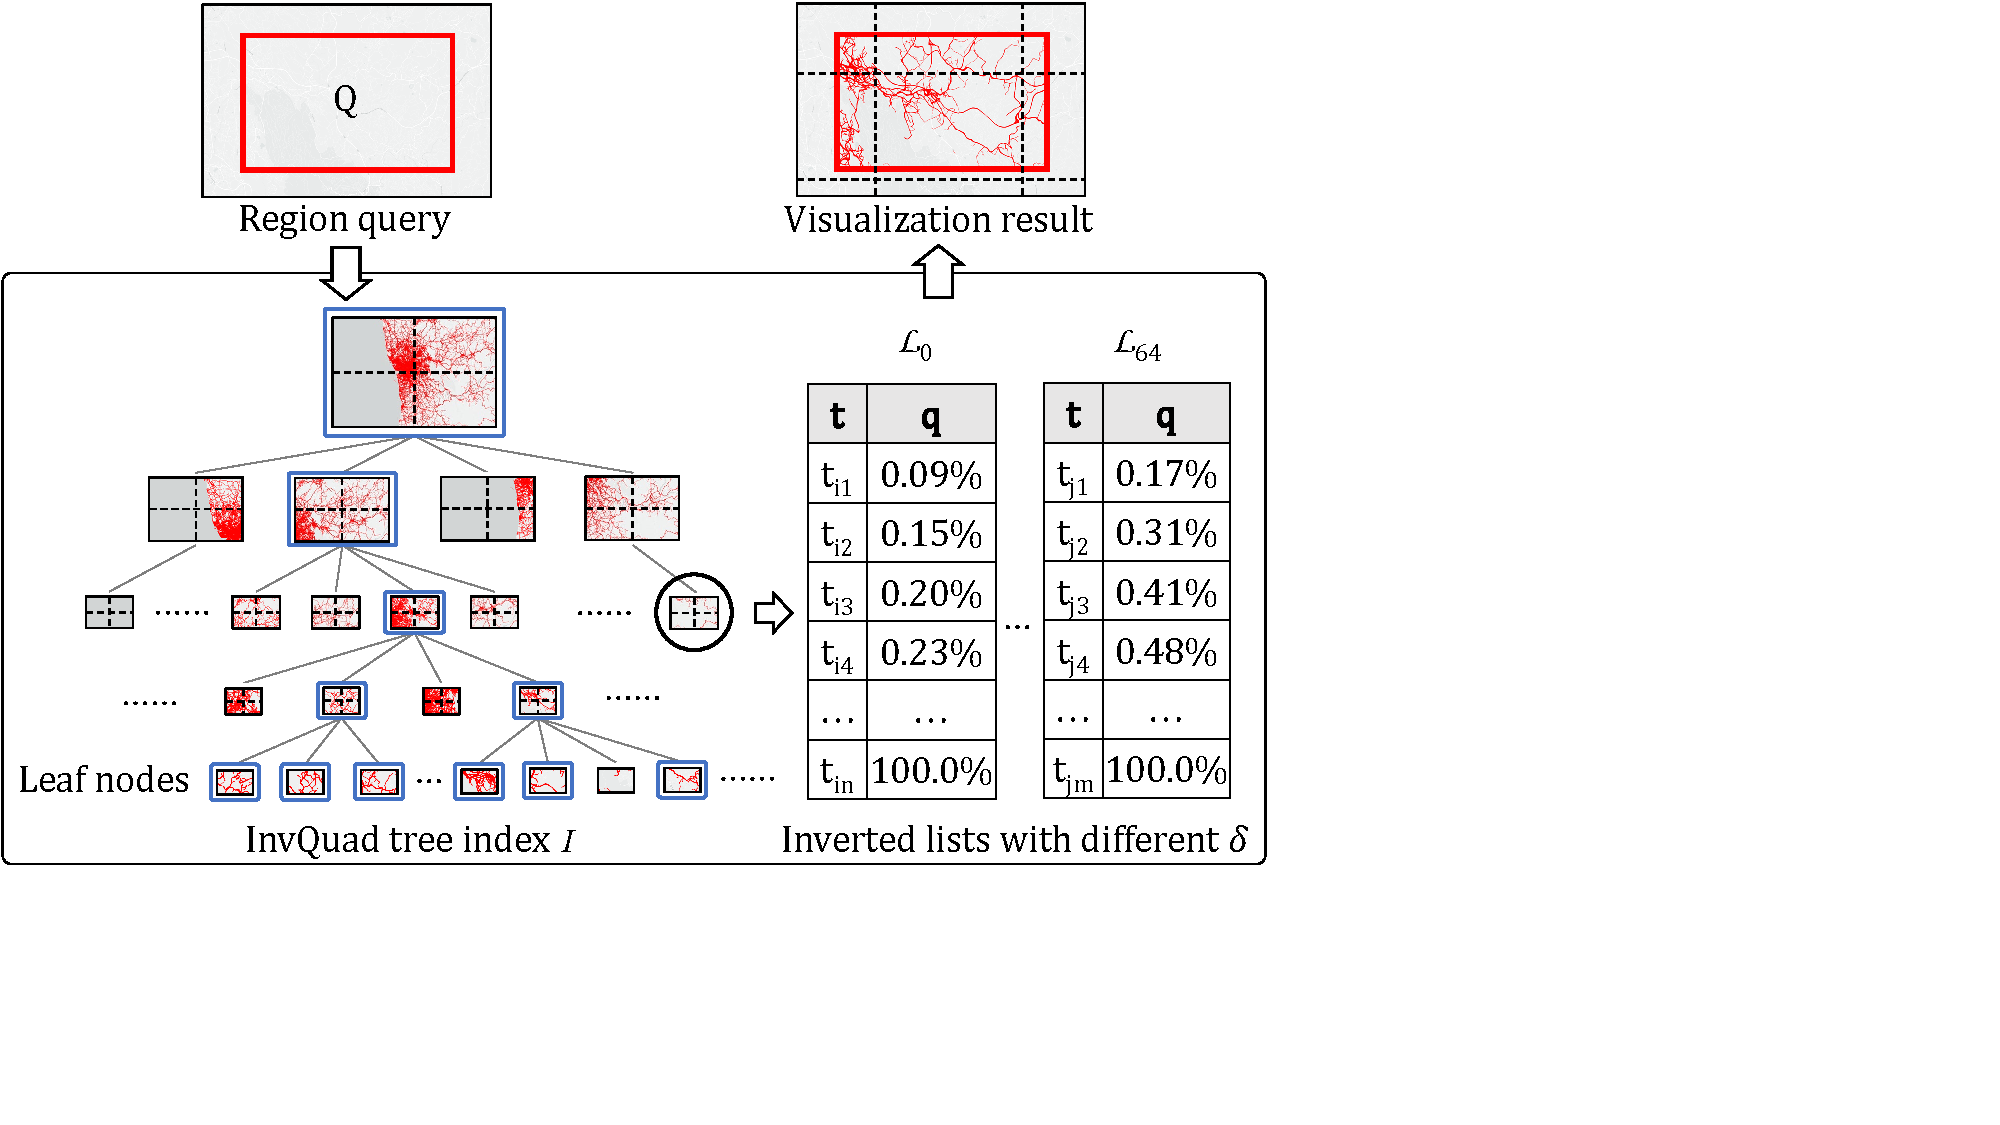
\includegraphics[width=0.4\textwidth]{pictures/cheetahtraj}
    \trim
    \caption{The $\avats$ framework.}
    \label{fig:framework}
    \trim
\end{figure}


\subsection{Index Building}~\label{sec:index}
The key idea of $\avats$ is to conduct $\vatss$ sampling in the offline \emph{index building} phase such that the sampling results can be used for online visualization. To handle arbitrary query region, we develop an inverted list augmented quad-tree index ($\invQ$).

As shown in the example $\invQ$-tree index $\II$ at the bottom of Figure~\ref{fig:framework}, we exploit a quad-tree to recursively partition the entire area (spanned by the trajectory dataset) into smaller areas and manage each area with a tree node.
For each tree node, we run $\vatss$ using the trajectories (or trajectory segments) in its associated area as input to compute the \textit{visualization quality inverted lists} for this area. $\mathcal{L}_0$ and $\mathcal{L}_{64}$ in Figure~\ref{fig:framework} are two example visualization quality inverted lists, in which the subscripts are the values of $\delta$ for this list.
Specifically, we compute several inverted lists with different $\delta$ values\footnote{We set $\delta$ as 0 (i.e., $\vats$), 4, 8, 16, 32, 64. We need quality inverted lists with different $\delta$ for one area as the area may be covered by query regions of different sizes, and we use lists with larger $\delta$ for larger query region as discussed in Section~\ref{subsec:VQGS+}.} to support the efficient quality guaranteed result visualization at various zoom levels.
For each inverted list, (i) $\vatss$ terminates until the quality of the sample set is $100\%$, i.e., the visualization result of the sample set is the same as the full dataset;
(ii) the trajectory selected at each iteration of $\vatss$ is stored in the inverted list with its \textit{cumulative quality} in ascending order. Take inverted list $\mathcal{L}_0$ in Figure~\ref{fig:framework} for example, $t_{i4}$ is the trajectory selected at the $4$th iteration,
$t_{i4}$'s cumulative quality is $0.23\%$, which means that the quality achieved by $\{t_{i1}, t_{i2}, t_{i3}, t_{i4}\}$ as a whole is $0.23\%$. With the quality inverted list, searching a quality guaranteed sample set for a query region can be conducted efficiently via binary search.


\subsection{Query Processing}~\label{sec:query}
For a region visualization query $\query$ with quality threshold $\tau$, Algorithm~\ref{alg:query} summarizes the $\mathsf{Query}$ subroutine, which finds a quality guaranteed trajectory sample set $\oR$. The algorithm starts by invoking $\mathsf{Query}(\query, \tau, \II.root, \oR=\emptyset)$, i.e., from the root of $\invQ$-tree index $\II$ with an empty result set $\oR$, and then transverses the tree nodes recursively. If node   $\mathcal{N}$ is a leaf node or its associated area is entirely contained in the query region, we retrieve a quality guaranteed trajectory set by calling subroutine $\mathsf{findRet}()$, which conducts binary search on the proper inverted list in $\mathcal{N}$ (Line~\ref{line:ret}). Otherwise, we call $\mathsf{Query}()$ on the four children nodes of $\mathcal{N}$ ( Line~\ref{line:valls}-\ref{line:valle}). Note that Some trajectories in $\oR$, the result returned by $\mathsf{Query}()$ for region $\query$, may have segments outside $\mathcal{Q}$,
we conduct a way point query $\wpts(\query, \oR)$ to filter these segments before visualization.


\begin{algorithm}
	\caption{$\mathsf{Query}$($\query$, $\tau$, $\invQ$ node $\mathcal{N}$, result $\oR$)}
	\label{alg:query}
	\begin{algorithmic}[1]
        \If{ $\mathcal{N}$ is leaf node or  $\mathcal{N}$ is entirely contained in $\query$}
            \State $\oR \leftarrow \oR \cup \mathsf{findRet}(\mathcal{N}, \tau)$ \label{line:ret}
        \ElsIf {$\query \cap \mathcal{N} \neq \emptyset$} \label{line:valls}
            \For { $i$ from $0$ to $3$}
                \State $\mathsf{tmpQ} \leftarrow \query \cap \mathcal{N}.child[i]$
                \State $\mathsf{Query}(\mathsf{tmpQ}, \tau, \mathcal{N}.child[i], \oR)$
            \EndFor \label{line:valle}
        \EndIf
	\end{algorithmic}
\end{algorithm}


%

\stitle{Correctness analysis}
We first show that $\avats$ meets the visualization quality requirement in Theorem~\ref{theorem:quality} as follows.
\begin{theorem}\label{theorem:quality}
If all selected nodes in the $\invQ$-tree index $\II$ are entirely contained in the query region $\query$,
then the result set $\oR$ returned by Algorithm~\ref{alg:query} satisfies that $\QQ(\oR) \ge \tau$.
\end{theorem}
\begin{proof}
Suppose query region $\query$ selects areas $\mathcal{A}_1,\!\mathcal{A}_2,\!\cdots,\!\mathcal{A}_K$,
these areas satisfy $\mathcal{A}_i \cap \mathcal{A}_j = \emptyset$ for $i\neq j$, and $\cup_{k=1}^{K}\mathcal{A}_k=\mathcal{Q}$.
For each area $\mathcal{A}_k$, denote the number of points marked in the ground truth visualization as $n_k$,
and the number of points marked by the trajectories in $\mathcal{R}$ as $m_k$,
we have $\frac{m_k}{n_k} \ge \tau$ as we use the visualization quality inverted index for trajectory selection.
Thus, for query region $\query$ with result set $\oR$, we have
$\QQ(\oR) = \frac{\sum_{k=1}^{K} m_k}{\sum_{k=1}^{K} n_k} \ge \tau.$
\end{proof}
In more general cases, we also select some areas that only intersect with the query region $\query$ and the sample set $\oR$ may not satisfy $\frac{m_k}{n_k}\ge \tau$ for these areas.
This does not significantly affect visualization quality for two reasons:
(i) these areas are the leaf nodes of the $\invQ$-tree index and thus reside on the border of the query region.
When exploring the map, human tends to move the region of interest to the screen center, where is more ``close'' to eyes~\cite{fitts_click}. %fitts,
(ii) the areas of the border regions are small w.r.t. the query region if the $\invQ$-tree has a sufficient height (i.e., the leaf nodes have a small area).

